\documentclass[10pt]{article}
\usepackage[letterpaper,margin=0.8in,top=0.6in,bottom=0.6in]{geometry}
\usepackage[T1]{fontenc}
\usepackage{tgpagella,mathpazo,tgheros}
\usepackage{amsmath,amssymb,booktabs,graphicx,xcolor,microtype,array,titlesec,enumitem,float}
\usepackage[font=small,labelfont={bf,sf},skip=5pt]{caption}
\usepackage{pgfplots}
\usepgfplotslibrary{groupplots}
\usetikzlibrary{arrows.meta,positioning,calc}
\pgfplotsset{compat=1.18}
\usepackage[colorlinks=true,urlcolor=blue!45!black,linkcolor=blue!45!black]{hyperref}
\hypersetup{pdftitle={Which module binds first in latent planning? A preliminary RoboJEPA diagnostic}}

\definecolor{real}{HTML}{1F5FA8}
\definecolor{bad}{HTML}{C0392B}
\definecolor{ok}{HTML}{1A8F7A}
\definecolor{warn}{HTML}{C77F00}
\definecolor{mute}{HTML}{7A7F87}

\setlength{\parindent}{0pt}\setlength{\parskip}{4pt}
\titleformat{\section}{\sffamily\bfseries\normalsize}{\thesection}{0.6em}{}
\titlespacing*{\section}{0pt}{5pt}{0pt}
\pagestyle{empty}
\newcommand{\zh}{\hat z}
\newcommand{\U}{\mathcal U}

\begin{document}

{\sffamily\bfseries\LARGE Which module binds first in latent planning?\par}
\vspace{2pt}
{\sffamily\large A preliminary RoboJEPA diagnostic\par}
\vspace{3pt}
{\sffamily\small\color{mute} Preliminary lab report \,$\cdot$\, 11 November 2026 \,$\cdot$\, one simulator context, released frozen models, no training\par}
\vspace{4pt}\hrule\vspace{5pt}

\textbf{Summary.} A latent world-model planner chains an encoder, a predictor, a goal cost and a search
procedure. On the released RoboJEPA model~[1], in one RoboCasa reach context with seven millimetre-scale
actions, the encoder and goal cost order actions by physical progress almost perfectly, while the predictor's
response to action is about thirty times too small and nearly orthogonal to the realized change. Fed the
commanded rather than the executed motion, the predictor also misorders the actions. The study therefore
turns to predictor sensitivity and the action interface before any comparison of optimizers.

\begin{figure}[H]
\begin{minipage}[b]{0.245\textwidth}
  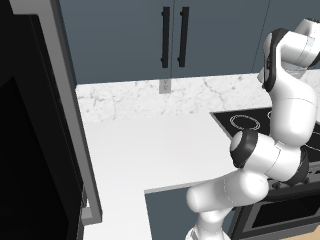
\includegraphics[width=\linewidth]{assets/base-side.png}\\[1pt]
  {\sffamily\scriptsize\textbf{(a)} Start state, side camera.}\\[5pt]
  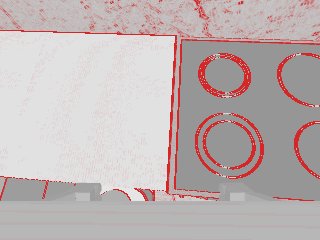
\includegraphics[width=\linewidth]{assets/diff-wrist.png}\\[1pt]
  {\sffamily\scriptsize\textbf{(b)} Wrist camera: pixels changed between start and goal, in red.}
\end{minipage}\hfill
\begin{minipage}[b]{0.73\textwidth}
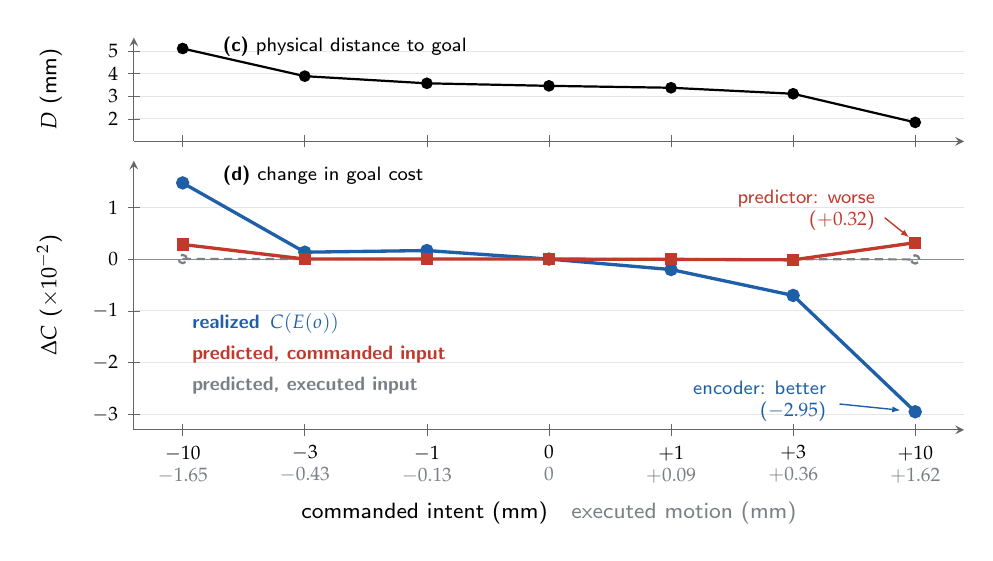
\begin{tikzpicture}[font=\sffamily\footnotesize]
\begin{groupplot}[
  group style={group size=1 by 2, vertical sep=7pt, x descriptions at=edge bottom},
  width=\linewidth, xmin=0.6, xmax=7.4, xtick={1,...,7},
  axis lines=left, axis line style={black!60}, tick style={black!60},
  ymajorgrids, grid style={black!10}, clip=false,
  tick label style={font=\sffamily\scriptsize}, label style={font=\sffamily\footnotesize}]
\nextgroupplot[height=2.9cm, ymin=1, ymax=5.6, ytick={2,3,4,5},
  ylabel={$D$ (mm)}, ylabel style={at={(axis description cs:-0.075,0.5)}}]
  \addplot[black, thick, mark=*, mark size=1.7pt] coordinates
    {(1,5.114)(2,3.889)(3,3.572)(4,3.460)(5,3.375)(6,3.109)(7,1.841)};
  \node[anchor=west, font=\sffamily\scriptsize] at (axis cs:1.25,5.2) {\textbf{(c)} physical distance to goal};
\nextgroupplot[height=5.0cm, ymin=-3.3, ymax=1.9, ytick={-3,-2,-1,0,1},
  ylabel={$\Delta C$ ($\times10^{-2}$)}, ylabel style={at={(axis description cs:-0.075,0.5)}},
  xticklabels={{$-10$\\\textcolor{mute}{$-1.65$}},{$-3$\\\textcolor{mute}{$-0.43$}},{$-1$\\\textcolor{mute}{$-0.13$}},
               {$0$\\\textcolor{mute}{$0$}},{$+1$\\\textcolor{mute}{$+0.09$}},{$+3$\\\textcolor{mute}{$+0.36$}},{$+10$\\\textcolor{mute}{$+1.62$}}},
  xticklabel style={align=center},
  xlabel={commanded intent (mm)\quad\textcolor{mute}{executed motion (mm)}}]
  \draw[black!45, line width=.4pt] (axis cs:0.6,0) -- (axis cs:7.4,0);
  \addplot[real, very thick, mark=*, mark size=1.8pt] coordinates
    {(1,1.4715)(2,0.1330)(3,0.1649)(4,0)(5,-0.2022)(6,-0.7025)(7,-2.9505)};
  \addplot[mute, thick, densely dashed, mark=o, mark size=1.5pt] coordinates
    {(1,0.0013)(2,0.0005)(3,-0.0002)(4,0)(5,-0.0003)(6,-0.0015)(7,-0.0064)};
  \addplot[bad, very thick, mark=square*, mark size=1.6pt] coordinates
    {(1,0.2823)(2,0.0012)(3,0.0032)(4,0)(5,-0.0054)(6,-0.0155)(7,0.3170)};
  \node[anchor=west, font=\sffamily\scriptsize] at (axis cs:1.25,1.62) {\textbf{(d)} change in goal cost};
  \node[anchor=west, real, font=\sffamily\scriptsize\bfseries] at (axis cs:1.0,-1.25) {realized \,$C(E(o))$};
  \node[anchor=west, bad, font=\sffamily\scriptsize\bfseries] at (axis cs:1.0,-1.85) {predicted, commanded input};
  \node[anchor=west, mute, font=\sffamily\scriptsize\bfseries] at (axis cs:1.0,-2.45) {predicted, executed input};
  \node[anchor=east, bad, font=\sffamily\scriptsize, align=right] at (axis cs:6.75,0.95) {predictor: worse\\($+0.32$)};
  \draw[bad, -{Latex[length=3pt]}, line width=.5pt] (axis cs:6.75,0.8) -- (axis cs:6.95,0.42);
  \node[anchor=east, real, font=\sffamily\scriptsize, align=right] at (axis cs:6.35,-2.75) {encoder: better\\($-2.95$)};
  \draw[real, -{Latex[length=3pt]}, line width=.5pt] (axis cs:6.38,-2.8) -- (axis cs:6.88,-2.92);
\end{groupplot}
\end{tikzpicture}
\end{minipage}
\caption{\textbf{The encoder sees millimetre progress; the predictor does not.} Seven actions along one ray;
the goal is the endpoint of a $+20$\,mm command on that ray (3.5\,mm of motion). \textbf{(c)} Distance to goal falls
monotonically and \textbf{(d)} the realized latent cost follows it. The predictor is flat given the executed
motion, and rises for both large moves given the commanded value.}
\end{figure}

\section{Three readings per action}
With history $h$, action $U$, frozen encoder $E$, predictor $F$ and goal feature $g$, every action receives
\begin{equation*}
\underbrace{C\big(F(h,U)\big)}_{\text{predicted}},\qquad
\underbrace{C\big(E(o(U))\big)}_{\text{realized}},\qquad
\underbrace{D(U)=\lVert x(U)-x_g\rVert_2}_{\text{physical}},\qquad C(z)=\tfrac1p\lVert z-g\rVert_1 .
\end{equation*}
The planner minimizes the first; the task is the third; the second isolates the predictor from the
representation and cost. A planner uses a cost only through the order it induces on actions, so
Table~\ref{tab:rank} scores each reading as a selector over the seven actions.

\begin{table}[H]\centering\small
\setlength{\tabcolsep}{7pt}
\begin{tabular}{@{}lccc@{}}
\toprule
Selector & Picks & Pairs ordered like $D$ & Progress captured \\
\midrule
Realized cost $C(E(o))$ & $+10$ & 20\,/\,21 & 1.62 of 1.62\,mm \\
Predicted, executed-motion input & $+10$ & 20\,/\,21 & 1.62 of 1.62\,mm \\
Predicted, commanded input & $+3$ & 14\,/\,21 & \textcolor{bad}{\textbf{0.35 of 1.62\,mm}} \\
\bottomrule
\end{tabular}
\caption{Each reading as an action selector. Executed-motion input uses the outcome, so it is unavailable when planning.}
\label{tab:rank}
\end{table}

\textbf{Representation and cost.} A 1.6\,mm move lowers the realized cost by 30\% ($0.0990\to0.0695$); a
repeated neutral trial moves it by $1.5\times10^{-6}$. \textbf{Predictor.} Given the executed motion, its
feature response is 3\% of the realized response (mean $|\Delta z|$ $0.0022$ against $0.072$) with cosine
$0.17$, and its cost change is 0.2\% of the realized one. The order survives; the amplitude does not.
\textbf{Action interface.} The pilot's fixed four-substep controller executed 1.6\,mm of a 10\,mm command.
The predictor's state-delta input describes executed motion, so the commanded value overstates it sixfold and
both large moves read as worse.

\begin{figure}[H]\centering
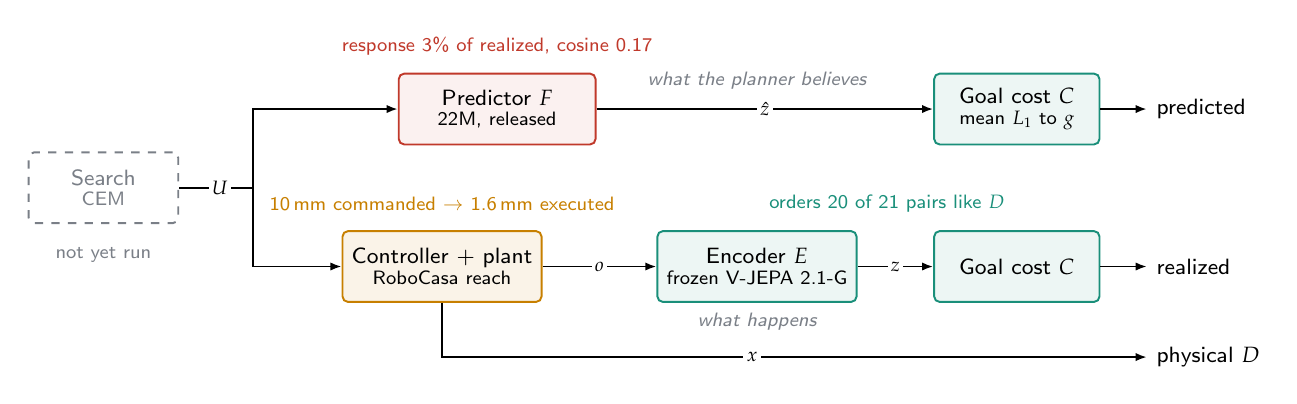
\begin{tikzpicture}[font=\sffamily\footnotesize, >={Latex[length=4pt]},
  box/.style={draw, rounded corners=2pt, minimum height=9mm, minimum width=25mm, align=center, line width=.7pt},
  chip/.style={font=\sffamily\scriptsize, align=center}, lab/.style={font=\sffamily\scriptsize, fill=white, inner sep=1.2pt}]
\node[box, dashed, draw=mute, text=mute, minimum width=19mm] (S) at (0,0) {Search\\[-2pt]{\scriptsize CEM}};
\node[box, draw=bad, fill=bad!7] (F) at (5.0,1.0) {Predictor $F$\\[-2pt]{\scriptsize 22M, released}};
\node[box, draw=warn, fill=warn!9] (P) at (4.3,-1.0) {Controller + plant\\[-2pt]{\scriptsize RoboCasa reach}};
\node[box, draw=ok, fill=ok!8] (E) at (8.3,-1.0) {Encoder $E$\\[-2pt]{\scriptsize frozen V-JEPA 2.1-G}};
\node[box, draw=ok, fill=ok!8, minimum width=21mm] (C1) at (11.6,1.0) {Goal cost $C$\\[-2pt]{\scriptsize mean $L_1$ to $g$}};
\node[box, draw=ok, fill=ok!8, minimum width=21mm] (C2) at (11.6,-1.0) {Goal cost $C$};
\node[anchor=west] (R1) at (13.25,1.0) {predicted};
\node[anchor=west] (R2) at (13.25,-1.0) {realized};
\node[anchor=west] (R3) at (13.25,-2.15) {physical $D$};
\coordinate (split) at (1.9,0);
\draw[line width=.7pt] (S) -- (split) node[lab, pos=.55] {$U$};
\draw[->, line width=.7pt] (split) |- (F);
\draw[->, line width=.7pt] (split) |- (P);
\draw[->, line width=.7pt] (F) -- (C1) node[lab, midway] {$\zh$};
\draw[->, line width=.7pt] (P) -- (E) node[lab, midway] {$o$};
\draw[->, line width=.7pt] (E) -- (C2) node[lab, midway] {$z$};
\draw[->, line width=.7pt] (C1) -- (R1);
\draw[->, line width=.7pt] (C2) -- (R2);
\draw[->, line width=.7pt] (P.south) |- (R3) node[lab, pos=.72] {$x$};
\node[chip, bad] at (5.0,1.8) {response 3\% of realized, cosine 0.17};
\node[chip, warn] at (4.3,-0.2) {10\,mm commanded $\to$ 1.6\,mm executed};
\node[chip, ok] at (9.95,-0.2) {orders 20 of 21 pairs like $D$};
\node[chip, mute] at (0,-0.85) {not yet run};
\node[font=\sffamily\scriptsize\itshape, mute] at (8.3,1.36) {what the planner believes};
\node[font=\sffamily\scriptsize\itshape, mute] at (8.3,-1.7) {what happens};
\end{tikzpicture}
\caption{\textbf{Where the chain holds and where it bends.} One action, scored by the predictor and by the
world. Colour is the status measured in this context: \textcolor{ok}{adequate}, \textcolor{warn}{mismatched
interface}, \textcolor{bad}{weak response}, \textcolor{mute}{untested}.}
\end{figure}

\section{Hypothesis}
Let $U_S$ be the action the search returns, and $U_F$, $U_E$, $U_\star$ the minimizers over a candidate set $\U$
of the predicted cost, the realized cost and $D$. Physical regret splits by module:
\begin{equation*}
D(U_S)-D(U_\star)=
\underbrace{D(U_S)-D(U_F)}_{\text{search}}
+\underbrace{D(U_F)-D(U_E)}_{\text{predictor and action interface}}
+\underbrace{D(U_E)-D(U_\star)}_{\text{representation and cost}} .
\end{equation*}
Measured here: the last term is $0$; the middle term is $1.27$\,mm with commanded input and $0$ with
executed input; the first is unmeasured. \textbf{We hypothesize that the middle term binds first in general}, and
that it has two separable causes: the meaning of $U$ at the interface, and the predictor's gain $G(a)=\Delta C\big(F(h,U_a)\big)\big/\Delta C\big(E(o(U_a))\big)$, measured here at $G\approx0.002$ for 1.6\,mm of executed motion.
Control improves by acting on the binding module; a stronger optimizer applied to a flat predictor returns
the same wrong action faster. Prior work shows that task success and faithful latent dynamics dissociate~[2];
the decomposition makes that dissociation measurable per module.

\section{Next experiment}
\textbf{Amplitude--ranking sweep} (not yet run). Eight independent start--goal instances; nine commands
from 1\,mm to 5\,cm along a fixed ray; the release's controller and action contract; predictions sealed
before execution. Each instance yields the curves of Fig.~1, the gain $G(a)$ and the three regret terms:
about 90 resets, roughly one GPU-hour at the measured 40\,s each.

\begin{table}[H]\centering\small
\setlength{\tabcolsep}{6pt}\renewcommand{\arraystretch}{1.12}
\begin{tabular}{@{}p{.36\textwidth}p{.25\textwidth}p{.31\textwidth}@{}}
\toprule
Outcome across instances & Binding module & Next move \\
\midrule
$G(a)\to1$ as amplitude reaches centimetres & predictor, small actions only & fine-scale feedback module around $F$ \\
$G(a)\ll1$ at every amplitude & predictor & larger checkpoint, or adapt $F$ \\
Realized cost misorders actions & representation and cost & goal metric \\
Both costs order correctly, search misses $U_F$ & search & CEM against gradient planners \\
\bottomrule
\end{tabular}
\caption{Decision table fixed before the sweep. Each row names one module and one move.}
\end{table}

\section{Evidence and scope}
\vspace{-6pt}
\begin{table}[H]\centering\footnotesize
\setlength{\tabcolsep}{5pt}\renewcommand{\arraystretch}{1.08}
\begin{tabular}{@{}p{.1\textwidth}p{.86\textwidth}@{}}
\toprule
Executed & 9 simulator resets, 29 Oct: 2 neutral, $\pm1$, $\pm3$, $\pm10$\,mm, and the $+20$\,mm goal. One scene, seed, start state and goal direction; horizon 0.2\,s. 7 candidate actions, 21 pairs; $p=998{,}400$ features per endpoint. \\
Models & Released 22M predictor (smallest) and frozen encoder. Nothing was trained or tuned, hence no train, validation or test split. \\
Choices & Scene, ray, magnitudes, goal and the four-substep controller were fixed by the pilot protocol before responses were read, not by the principal investigator. No trial is excluded. \\
Recomputed & Every number above, from the raw arrays (\texttt{recompute.py} $\to$ \texttt{evidence.json}). The ranking statistics are new and post hoc. \\
Scope & One context gives an instrument and a direction, not a rate. All seven actions lie on the ray through the goal, so the ordering test probes one direction. Executed motion of at most 1.7\,mm is small against the release's 5\,cm command normalization, so the measured gain may describe a small-action regime. \\
Not run & Any planner; other scenes, seeds or goals; centimetre actions; larger checkpoints; command-conditioned input; the release's blocking controller; a real robot. \\
\bottomrule
\end{tabular}
\end{table}

\vspace{-6pt}{\footnotesize
[1] A.~Zholus et al. \emph{RoboJEPA: Scaling Robotic Latent World Models}. \href{https://arxiv.org/abs/2610.10515}{arXiv:2610.10515}, 2026.\quad
[2] R.~Gonzalez Laiz, S.~Schneider. \emph{Understanding the Limits of Latent World Models}. \href{https://arxiv.org/abs/2610.37588}{arXiv:2610.37588}, 2026.}

\end{document}
